% !TEX root = ../../../main.tex
\pgfplotsset{compat=newest}
\begin{figure}
    \centering
      \subfigure[函数最优解落在可行域之内]{
    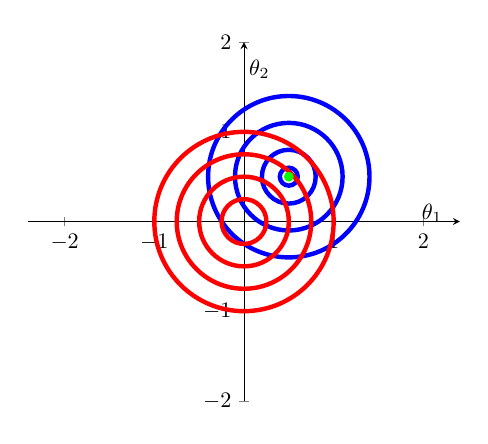
\begin{tikzpicture}[scale=0.8]
        \begin{axis}[
         axis lines=middle,
                axis equal,
         xmin=-2, xmax=2, ymin=-2, ymax=2,
         every axis x label/.style={at={(current axis.right of origin)},anchor=west,above=2em,right=1.5em},
         every axis y label/.style={at={(current axis.north)},above=2em,right=1.5em},
        xlabel = $\theta_1$,
        ylabel = $\theta_2$
        ]
        \draw [blue, line width=2pt](axis cs: 0.5, 0.5) circle [radius=0.1];
        \draw [blue, line width=2pt](axis cs: 0.5, 0.5) circle [radius=0.3];
        \draw [blue, line width=2pt](axis cs: 0.5, 0.5) circle [radius=0.6];
        \draw [blue, line width=2pt](axis cs: 0.5, 0.5) circle [radius=0.9];

        \draw [red, line width=2pt](axis cs: 0, 0) circle [radius=1];
        \draw [red, line width=2pt](axis cs: 0, 0) circle [radius=0.75];
        \draw [red, line width=2pt](axis cs: 0, 0) circle [radius=0.5];
        \draw [red, line width=2pt](axis cs: 0, 0) circle [radius=0.25];
        \addplot[green,only marks] coordinates{(0.5, 0.5)};
        \end{axis}
    \end{tikzpicture}
            
            }
    \subfigure[函数最优解落在可行域之外]{
    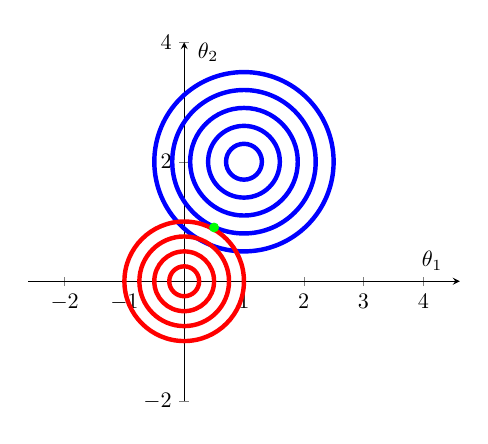
\begin{tikzpicture}[scale=0.8]
    \begin{axis}[
        axis equal,
         axis lines=middle,
         xmin=-2, xmax=4, ymin=-2, ymax=4,
        xlabel = $\theta_1$,
        ylabel = $\theta_2$,
        every axis x label/.style={at={(current axis.right of origin)},anchor=west,above=2em,right=1.5em},
         every axis y label/.style={at={(current axis.north)},above=2em},
        ]
        \draw [blue, line width=2pt](axis cs: 1, 2) circle [radius=0.3];
        \draw [blue, line width=2pt](axis cs: 1, 2) circle [radius=0.6];
        \draw [blue, line width=2pt](axis cs: 1, 2) circle [radius=0.9];
        \draw [blue, line width=2pt](axis cs: 1, 2) circle [radius=1.2];
        \draw [blue, line width=2pt](axis cs: 1, 2) circle [radius=1.5];

        \draw [red, line width=2pt](axis cs: 0, 0) circle [radius=1];
        \draw [red, line width=2pt](axis cs: 0, 0) circle [radius=0.75];
        \draw [red, line width=2pt](axis cs: 0, 0) circle [radius=0.5];
        \draw [red, line width=2pt](axis cs: 0, 0) circle [radius=0.25];
        \addplot[green, only marks] coordinates{(0.5, 0.9)};

    \end{axis}
	\end{tikzpicture}
            }
          
\caption{不等式约束下的极值问题\label{fig:L2_lang}}
\end{figure}
